% =============================================================================
% PRESENTACIÓN CANDIDATURA DOCTORAL - V4 (INTEGRACIÓN COMPLETA DEB)
% Una diapositiva, un tema. Bloque técnico DEB integrado.
% =============================================================================

\documentclass[aspectratio=169, 11pt]{beamer}

% --- Fuentes (XeLaTeX) ---
\usepackage{fontspec}
\setmainfont{TeX Gyre Termes}
\setsansfont{TeX Gyre Heros}
\setmonofont{Latin Modern Mono}

\usepackage[spanish,es-nodecimaldot]{babel}
\usepackage{amsmath, amssymb}
\usepackage{booktabs}
\usepackage{graphicx}
\usepackage{tikz}
\usetikzlibrary{shapes.geometric, arrows.meta, positioning, calc, fit, shadows, shapes.symbols}

% --- Tema ---
\usetheme{Madrid}
\usecolortheme{beaver}
\definecolor{unalRojo}{RGB}{148, 36, 36}
\definecolor{verdeOK}{RGB}{34, 139, 34}
\definecolor{naranjaAlerta}{RGB}{230, 126, 34}
\definecolor{rojoAlerta}{RGB}{192, 57, 43}
\setbeamercolor{structure}{fg=unalRojo}
\setbeamercolor{block title}{bg=unalRojo!15, fg=unalRojo}
\setbeamercolor{block body}{bg=unalRojo!5}
\setbeamercolor{alerted text}{fg=rojoAlerta}

% --- Metadatos ---
\title[Sistema Híbrido BSF]{Sistema Híbrido para Predicción de Emisiones}
\subtitle{CO$_2$ y CH$_4$ en Bioconversión con \textit{Hermetia illucens}}
\author{John Jairo Leal Gómez}
\institute[UNAL]{Doctorado en Estudios Ambientales\\Universidad Nacional de Colombia -- Sede Palmira}
\date{Abril 2026}
\titlegraphic{
\includegraphics[width=1.5cm]{../tesis/00Figuras/00f00EscudoUN2016.jpg}}

% --- Comandos ---
\newcommand{\BSF}{\textit{Hermetia illucens}}
\newcommand{\MAPE}{\text{MAPE}}
\newcommand{\DEB}{\text{DEB}}
\newcommand{\NDIR}{\text{NDIR}}

\setbeamertemplate{navigation symbols}{}
\setbeamertemplate{footline}[frame number]

\begin{document}

% =============================================================================
% APERTURA
% =============================================================================

\begin{frame}[plain]
    \titlepage
\end{frame}

\begin{frame}{Índice de la Presentación}
    \tableofcontents
\end{frame}

% =============================================================================
% SECCIÓN 1: EL PROBLEMA CLIMÁTICO
% =============================================================================
\section{El Problema Climático}

\begin{frame}{Concentraciones Récord de GEI en 2024}
    Según el WMO Greenhouse Gas Bulletin No. 21:
    \begin{itemize}
        \item \textbf{CO$_2$:} 423.9 ppm (nivel sin precedentes en la historia humana)
        \item \textbf{CH$_4$:} 1942 ppb (potencial de calentamiento global 28$\times$ superior al CO$_2$)
        \item \textbf{N$_2$O:} 338.0 ppb
    \end{itemize}
    \vspace{0.3cm}
    \centering
    \footnotesize \textit{Fuente: WMO, 2025.}
\end{frame}

\begin{frame}{Concentraciones Récord de GEI (Visualización)}
    \centering
    \begin{tikzpicture}[scale=0.9]
        \fill[unalRojo!30] (0,0) rectangle (1.2,4.239);
        \fill[naranjaAlerta!50] (2,0) rectangle (3.2,1.942);
        \fill[verdeOK!40] (4,0) rectangle (5.2,1.5);
        \node[below, font=\small] at (0.6,0) {CO$_2$};
        \node[below, font=\small] at (2.6,0) {CH$_4$};
        \node[below, font=\small] at (4.6,0) {N$_2$O};
        \node[above, font=\tiny, rotate=90, anchor=south] at (0.6,2.1) {423.9 ppm};
        \node[above, font=\tiny, rotate=90, anchor=south] at (2.6,0.9) {1942 ppb};
        \draw[->, thick] (-0.5,0) -- (6,0) node[right, font=\small] {Gas};
        \draw[->, thick] (-0.5,0) -- (-0.5,5) node[above, font=\small] {Concentración};
    \end{tikzpicture}
\end{frame}

\begin{frame}{La Paradoja del 0.042\%}
    No se trata de abundancia relativa, sino de \textbf{propiedades radiativas intrínsecas} de la molécula de CO$_2$.
    \vspace{0.3cm}
    \begin{itemize}
        \item Absorbe y reemite eficazmente la radiación infrarroja térmica
        \item El forzamiento radiativo se ha alterado irreversiblemente
        \item Eventos climáticos extremos, pérdida de biodiversidad, saturación de sumideros naturales
    \end{itemize}
\end{frame}

\begin{frame}{Gestión de Residuos en el Sur Global}
    Más del 50\% de los residuos sólidos en países de ingresos medios y bajos son orgánicos.
    \vspace{0.3cm}
    \begin{itemize}
        \item Dispersión geográfica y estacionalidad de la generación
        \item Alta carga biodegradable (especialmente en zonas agroindustriales)
        \item Infraestructura de tratamiento limitada o inexistente
    \end{itemize}
    \vspace{0.3cm}
    \centering
    \footnotesize \textit{Contexto Valle del Cauca: residuos de café, caña y frutas.}
\end{frame}

\begin{frame}{Limitaciones de las Soluciones Convencionales}
    \begin{itemize}
        \item \textbf{Rellenos sanitarios:} Emisiones prolongadas y difusas de CH$_4$ durante años o décadas
        \item \textbf{Digestión anaerobia:} Infraestructura compleja, costosa, inviable a pequeña escala
        \item \textbf{Compostaje:} Emisiones de N$_2$O y tiempos largos de estabilización
    \end{itemize}
    \vspace{0.3cm}
    En contextos agroindustriales del Sur Global, estas alternativas resultan técnicamente o económicamente inviables.
\end{frame}

% =============================================================================
% SECCIÓN 2: BSF
% =============================================================================
\section{Bioconversión con \textit{Hermetia illucens}}

\begin{frame}{\BSF{}: De Residuo a Recurso}
    La bioconversión con mosca soldado negra opera bajo un enfoque de economía circular:
    \vspace{0.3cm}
    \begin{itemize}
        \item \textbf{Entrada:} Residuos orgánicos agroindustriales
        \item \textbf{Proceso:} Larvas en estadios voraces (L3--L5), simbiosis con microbiota
        \item \textbf{Salidas:} Biomasa rica en proteínas y lípidos + frass (fertilizante orgánico)
    \end{itemize}
    \vspace{0.3cm}
    Reducción de masa: 50--80\% (base húmeda). Incremento larval: hasta 4000$\times$ su masa inicial.
\end{frame}

\begin{frame}{\BSF{}: Diagrama del Proceso}
    \centering
    \begin{tikzpicture}[scale=0.85, transform shape,
        caja/.style={rectangle, rounded corners, draw, minimum width=2.8cm, minimum height=1.2cm, align=center, font=\small}]
        \node[caja, fill=green!15] (res) at (0,3) {Residuos\\Orgánicos};
        \node[caja, fill=orange!15] (lar) at (0,1.2) {Larvas \BSF\\(Metabolismo)};
        \node[caja, fill=blue!15] (bio) at (-3,0) {Biomasa\\(Proteína/Lípidos)};
        \node[caja, fill=brown!20] (fra) at (3,0) {Frass\\(Fertilizante)};
        \draw[->, thick, >=stealth] (res) -- (lar);
        \draw[->, thick, >=stealth] (lar) -- (bio);
        \draw[->, thick, >=stealth] (lar) -- (fra);
        \node[right=0.3cm of lar, font=\footnotesize, text=gray] {CO$_2$ + Calor};
    \end{tikzpicture}
\end{frame}

\begin{frame}{Ventajas Comparativas de la Bioconversión con BSF}
    Comparada con métodos tradicionales:
    \vspace{0.3cm}
    \begin{itemize}
        \item Requiere menor infraestructura
        \item Opera en tiempos cortos (3--4 semanas)
        \item Sin generación de lixiviados contaminantes
        \item Productos de valor agregado (proteína, fertilizante)
        \item Operable a pequeña escala en contextos rurales
    \end{itemize}
\end{frame}

\begin{frame}{El Problema de la ``Caja Negra''}
    A pesar del potencial, existe un vacío crítico de información:
    \vspace{0.3cm}
    \begin{itemize}
        \item Se conocen entradas (residuos) y salidas (biomasa, frass)
        \item Se desconocen los flujos gaseosos intermedios
        \item No existen factores de emisión específicos para BSF en el IPCC ni en el GHG Protocol
    \end{itemize}
\end{frame}

\begin{frame}{El Problema de la ``Caja Negra'' (Diagrama)}
    \centering
    \begin{tikzpicture}[scale=0.8, transform shape]
        \node[draw, dashed, rounded corners, fill=gray!10, minimum width=3.5cm, minimum height=3.5cm, align=center, font=\large] (caja) at (0,0) {?};
        \node[fill=green!20, rounded corners, minimum width=2cm, minimum height=1cm, font=\small] (in) at (-4.5,0) {Residuos};
        \node[fill=blue!20, rounded corners, minimum width=2cm, minimum height=1cm, font=\small] (out1) at (4.5,1.2) {Biomasa};
        \node[fill=brown!20, rounded corners, minimum width=2cm, minimum height=1cm, font=\small] (out2) at (4.5,-1.2) {Frass};
        \draw[->, thick, >=stealth] (in) -- (caja);
        \draw[->, thick, >=stealth] (caja) -- (out1);
        \draw[->, thick, >=stealth] (caja) -- (out2);
        \node[font=\footnotesize, text=red!70!black] at (0,-2.2) {CH$_4$ fugitivo?};
        \node[font=\footnotesize, text=red!70!black] at (0,-2.7) {CO$_2$ real?};
    \end{tikzpicture}
\end{frame}

\begin{frame}{Riesgo de Greenwashing}
    Sin monitoreo riguroso:
    \vspace{0.3cm}
    \begin{itemize}
        \item Cualquier balance de carbono se basa en supuestos no verificados
        \item BSF podría emitir más CH$_4$ que el compostaje en condiciones de anaerobiosis no controlada
        \item Se corre el riesgo de asignar beneficios climáticos no reales a la tecnología
        \item Ausencia de sistemas MRV impide acceso a mercados de carbono
    \end{itemize}
\end{frame}

% =============================================================================
% SECCIÓN 3: SISTEMA HÍBRIDO
% =============================================================================
\section{La Propuesta: Sistema Híbrido}

\begin{frame}{¿Por qué un Sistema Híbrido?}
    Ningún componente por sí solo puede validar la sostenibilidad ambiental del proceso.
    \vspace{0.3cm}
    \begin{itemize}
        \item \textbf{Sensores:} Capturan la realidad física pero carecen de contexto biológico (``ceguera semántica'')
        \item \textbf{Modelos EDO:} Aportan coherencia teórica pero fallan ante variabilidad biológica no parametrizada (``rigidez'')
        \item \textbf{IA pura:} Potente pero opaca, propensa al sobreajuste, sin restricciones físicas
    \end{itemize}
\end{frame}

\begin{frame}{¿Por qué un Sistema Híbrido? (Diagrama)}
    \centering
    \begin{tikzpicture}[scale=0.85, transform shape,
        comp/.style={rectangle, rounded corners, draw, minimum width=3.2cm, minimum height=1.2cm, align=center, font=\small\bfseries},
        flecha/.style={->, thick, >=stealth}]
        \node[comp, fill=gray!15] (sens) at (0,2.8) {Sensores IoT};
        \node[comp, fill=blue!10] (edo) at (-3.8,0) {Modelo EDO/DEB};
        \node[comp, fill=orange!10] (ia) at (3.8,0) {Aprendizaje Automático};
        \node[comp, fill=unalRojo!15, draw=unalRojo, line width=1.5pt] (hibr) at (0,-2.5) {SISTEMA HÍBRIDO};
        \draw[flecha] (sens) -- (edo);
        \draw[flecha] (sens) -- (ia);
        \draw[flecha] (edo) -- (hibr);
        \draw[flecha] (ia) -- (hibr);
        \draw[flecha, dashed] (edo) -- node[above, font=\tiny] {Corrección} (ia);
        \node[below=0.1cm of sens, font=\tiny, text=gray] {``Ceguera semántica''};
        \node[left=0.1cm of edo, font=\tiny, text=gray, align=right] {``Rigidez''};
        \node[right=0.1cm of ia, font=\tiny, text=gray, align=left] {``Opacidad''};
    \end{tikzpicture}
\end{frame}

\begin{frame}{Arquitectura en Cascada: Inferencia Biométrica}
    \textbf{Etapa 1 -- Red Neuronal (RNA):}
    \vspace{0.3cm}
    \begin{itemize}
        \item Entradas: temperatura, humedad, histórico de emisiones
        \item Salida: biomasa húmeda $W(t)$ y estadio larval \textit{en tiempo real}
        \item Resuelve el problema de que la medición directa es invasiva e impracticable
    \end{itemize}
\end{frame}

\begin{frame}{Arquitectura en Cascada: Modelado Metabólico}
    \textbf{Etapa 2 -- Modelo DEB Parametrizado:}
    \vspace{0.3cm}
    \begin{itemize}
        \item Desagregación matemática del flujo energético del organismo
        \item CO$_2$ = costo de mantenimiento somático + costo de síntesis de tejido
        \item Supuesto de trabajo: aerobiosis estricta
        \item Genera la línea base teórica: ``¿cuánto CO$_2$ debería emitir el sistema?''
    \end{itemize}
\end{frame}

\begin{frame}{Arquitectura en Cascada: Diagnóstico por Contrastación}
    \textbf{Etapa 3 -- Comparación Sensor vs. Modelo:}
    \vspace{0.3cm}
    \begin{equation*}
        Y_{sensor} = Y_{modelo} + \delta_{bio} + \epsilon_{inst}
    \end{equation*}
    \begin{itemize}
        \item $\epsilon_{inst}$: error instrumental (acotado por calibración)
        \item $\delta_{bio}$: desviación biológica (ineficiencia metabólica)
        \item Si divergencia $>$ umbral y CH$_4$ detectado $\Rightarrow$ \textbf{anaerobiosis}
    \end{itemize}
\end{frame}

\begin{frame}{Arquitectura en Cascada (Diagrama)}
    \centering
    \begin{tikzpicture}[scale=0.75, transform shape,
        etapa/.style={rectangle, rounded corners, draw, minimum width=3cm, minimum height=1.2cm, align=center, font=\small}]
        \node[etapa, fill=orange!15] (rna) at (0,3.5) {RNA\\$W(t)$ estimada};
        \node[etapa, fill=blue!10] (deb) at (0,1.8) {Modelo DEB\\$Y_{CO_2}$ teórico};
        \node[etapa, fill=red!10] (diag) at (0,0) {Diagnóstico\\Alerta};
        \node[left=0.8cm of rna, font=\footnotesize, align=right] {T, HR,\\CO$_2$ hist.};
        \node[right=0.8cm of diag, font=\footnotesize, align=left] {Verde / Ámbar / Rojo};
        \draw[->, thick, >=stealth] (rna) -- (deb);
        \draw[->, thick, >=stealth] (deb) -- (diag);
        \draw[->, thick, dashed] (rna.west) to[bend left=25] node[left, font=\tiny] {Real} (diag.west);
    \end{tikzpicture}
\end{frame}

% =============================================================================
% BLOQUE TÉCNICO: MODELO DEB (INTEGRADO DE PRESENTACION.TEX)
% =============================================================================

\begin{frame}{Flujo Metabólico DEB: Lógica del Carbono}
    El alimento entra al pool de \textbf{Asimilados ($A$)} y se distribuye en tres destinos.
    El CO$_2$ se genera como ``costo energético'' en cada punto:
    \vspace{0.3cm}
    \begin{itemize}
        \item \textbf{$r_{CO2,m}$:} Mantenimiento (costo fijo de vivir)
        \item \textbf{$r_{CO2,B}$:} Estructura (costo de crecer)
        \item \textbf{$r_{CO2,L}$:} Lípidos (costo de acumular reservas)
    \end{itemize}
\end{frame}

\begin{frame}{Flujo Metabólico DEB (Diagrama)}
    \centering
    \begin{tikzpicture}[scale=0.8, transform shape,
        caja/.style={rectangle, draw, thick, rounded corners, fill=white, align=center, font=\footnotesize\bfseries, minimum height=0.9cm, drop shadow},
        gas/.style={rectangle, draw, dashed, thick, fill=gray!5, minimum width=4cm, minimum height=0.7cm, font=\small}]
        \draw[fill=gray!10, draw=none, rounded corners=12pt] (-3.5, -1.4) rectangle (3.5, 1.4);
        \node[gray!50, font=\tiny, anchor=south] at (0,-1.4) {Larva};
        \node[caja, text width=1.8cm] (A) at (0, 0) {Asimilados\\$A$};
        \node[caja, text width=1.8cm] (B) at (-3, 0) {Estructura\\$B$};
        \node[caja, text width=1.8cm] (L) at (3, 0) {Lípidos\\$L$};
        \node[gas] (CO2) at (0, 2.5) {\Large CO$_2$};
        \draw[->, thick, >=stealth] (0, -1.4) -- node[fill=white, inner sep=1pt, font=\tiny] {$r_A$} (A);
        \draw[->, thick, >=stealth] (A) -- node[below, font=\tiny] {$r_B$} (B);
        \draw[->, thick, >=stealth] ([yshift=1.5mm]A.east) -- node[above, font=\tiny] {$r_L$} ([yshift=1.5mm]L.west);
        \draw[->, thick, >=stealth, dashed] ([yshift=-1.5mm]L.west) -- ([yshift=-1.5mm]A.east);
        \draw[->, thick, >=stealth] (A.north) -- node[fill=white, inner sep=1pt, font=\tiny] {$r_{CO2,m}$} (CO2.south);
        \draw[->, thick, >=stealth] (-1.5, 0.2) -- (-1.5, 2.1) node[midway, fill=white, inner sep=1pt, font=\tiny] {$r_{CO2,B}$};
        \draw[->, thick, >=stealth] (1.5, 0.2) -- (1.5, 2.1) node[midway, fill=white, inner sep=1pt, font=\tiny] {$r_{CO2,L}$};
    \end{tikzpicture}
\end{frame}

\begin{frame}{Ecuación Maestra del CO$_2$}
    Lo que mide el sensor es la suma de tres procesos fisiológicos:
    \vspace{0.3cm}
    \begin{equation*}
        r_{CO2} = \underbrace{r_{CO2,m}}_{\text{Mantenimiento}} + \underbrace{r_{CO2,B}}_{\text{Crecimiento}} + \underbrace{r_{CO2,L}}_{\text{Reservas (Grasa)}}
    \end{equation*}
    \vspace{0.3cm}
    El reto: el sensor entrega el total. El sistema debe ``desmezclar'' la señal para distinguir si las larvas están creciendo o solo manteniendo metabolismo basal.
\end{frame}

\begin{frame}{Asimilación y Apetito ($r_A$)}
    La producción de gas empieza por la boca. La ingesta depende del tamaño larval:
    \vspace{0.3cm}
    \begin{columns}[T]
        \column{0.48\textwidth}
        \textbf{Fase Exponencial}
        $$ r_A = a \cdot B $$
        \small La ingesta es proporcional al tamaño ($B$).
        
        \column{0.48\textwidth}
        \textbf{Freno de Saciedad}
        $$ a = a_{max} \left( 1 - \left( \frac{B}{B_{max}} \right)^\alpha \right) $$
        \small Cuando $B \to B_{max}$, la larva deja de comer.
    \end{columns}
    \vspace{0.3cm}
    \begin{alertblock}{Interpretación del Sensor}
        Si el CO$_2$ cae repentinamente, puede ser saciedad ($B_{max}$ alcanzado) y no falta de oxígeno.
    \end{alertblock}
\end{frame}

\begin{frame}{Dinámica de Lípidos ($r_L$): El Tanque de Reserva}
    A diferencia de la estructura ($B$) que siempre crece, los lípidos ($L$) funcionan como una batería: se cargan o se descargan.
    \vspace{0.3cm}
    \begin{block}{Balance de Energía}
        $$ r_L = \frac{r_A - (r_B + r_{CO2,m} + r_{CO2,B})}{1 + Y_L} $$
    \end{block}
    \vspace{0.2cm}
    \begin{columns}[T]
        \column{0.5\textwidth}
        \textbf{Superávit ($r_L > 0$)}\\
        \small Exceso guardado como aceite. \textcolor{verdeOK}{\textbf{$\rightarrow$ Acumulación}}
        \column{0.5\textwidth}
        \textbf{Déficit ($r_L < 0$)}\\
        \small Reservas quemadas para mantenerse viva. \textcolor{rojoAlerta}{\textbf{$\rightarrow$ Movilización}}
    \end{columns}
\end{frame}

\begin{frame}{Costo de Mantenimiento ($r_{CO2,m}$)}
    \centering
    \textbf{¿Cuánto ``cuesta'' simplemente existir?}
    \vspace{0.2cm}
    \begin{tikzpicture}[
        node distance=1.2cm,
        process/.style={rectangle, draw=red!80, fill=red!10, thick, rounded corners, minimum height=1cm, minimum width=2.5cm, align=center},
        input/.style={rectangle, draw=none, fill=blue!10, text=blue!60!black, font=\bfseries},
        status/.style={rectangle, draw=none, fill=green!10, text=green!60!black, font=\bfseries},
        gas/.style={cloud, draw=gray, fill=gray!10, aspect=2, minimum width=1.5cm, font=\small},
        arrow/.style={->, ultra thick, >=stealth, color=black!70}
    ]
        \node[process] (mach) {\textbf{Metabolismo Basal}};
        \node[input, left=0.8cm of mach] (in) {Biomasa ($B$)};
        \node[status, right=0.8cm of mach] (out) {Vida};
        \node[gas, above=0.8cm of mach] (co2) {CO$_2$};
        \draw[arrow] (in) -- (mach);
        \draw[arrow] (mach) -- (out);
        \draw[arrow, dashed, color=red!60!black] (mach) -- node[midway, right, font=\footnotesize, text=red!70!black] {Gasto ($m$)} (co2);
    \end{tikzpicture}
    \vspace{0.2cm}
    \begin{block}{Ecuación del Mantenimiento}
        \centering \large $ r_{CO2,m} = m \cdot B $
    \end{block}
    \small Este componente \textbf{nunca es cero} y aumenta linealmente con el tamaño.
\end{frame}

\begin{frame}{Costo de Crecer ($r_{CO2,B}$)}
    \centering
    \textbf{¿Cuánto ``cuesta'' fabricar nuevo tejido?}
    \vspace{0.2cm}
    \begin{tikzpicture}[
        node distance=1.2cm,
        process/.style={rectangle, draw=blue!80, fill=blue!10, thick, rounded corners, minimum height=1cm, minimum width=2.5cm, align=center},
        input/.style={rectangle, draw=none, fill=green!10, text=green!30!black, font=\bfseries},
        output/.style={rectangle, draw=none, fill=blue!20, text=blue!60!black, font=\bfseries},
        gas/.style={cloud, draw=gray, fill=gray!10, aspect=2, minimum width=1.5cm, font=\small},
        arrow/.style={->, ultra thick, >=stealth, color=black!70}
    ]
        \node[process] (mach) {\textbf{Anabolismo}};
        \node[input, left=0.8cm of mach] (in) {Aminoácidos};
        \node[output, right=0.8cm of mach] (out) {Tejido ($r_B$)};
        \node[gas, above=0.8cm of mach] (co2) {CO$_2$};
        \draw[arrow] (in) -- (mach);
        \draw[arrow] (mach) -- (out);
        \draw[arrow, dashed, color=red!60!black] (mach) -- node[midway, right, font=\footnotesize, text=red!70!black] {Costo ($Y_B$)} (co2);
    \end{tikzpicture}
    \vspace{0.2cm}
    \begin{block}{Ecuación del Crecimiento}
        \centering \large $ r_{CO2,B} = Y_B \cdot r_B $
    \end{block}
    \small A diferencia de la grasa, este componente \textbf{cae a cero} cuando la larva madura.
\end{frame}

\begin{frame}{Relación Estequiométrica ($Y_L$)}
    \centering
    \textbf{¿Por qué la producción de grasa genera gas?}
    \vspace{0.2cm}
    \begin{tikzpicture}[
        node distance=1.2cm,
        process/.style={rectangle, draw=blue!80, fill=blue!5, thick, rounded corners, minimum height=1cm, minimum width=2.5cm, align=center},
        input/.style={rectangle, draw=none, fill=green!10, text=green!30!black, font=\bfseries},
        output/.style={rectangle, draw=none, fill=orange!10, text=orange!60!black, font=\bfseries},
        gas/.style={cloud, draw=gray, fill=gray!10, aspect=2, minimum width=1.5cm, font=\small},
        arrow/.style={->, ultra thick, >=stealth, color=black!70}
    ]
        \node[process] (mach) {\textbf{Biosíntesis}};
        \node[input, left=0.8cm of mach] (in) {Nutrientes};
        \node[output, right=0.8cm of mach] (out) {Lípidos ($r_L$)};
        \node[gas, above=0.8cm of mach] (co2) {CO$_2$};
        \draw[arrow] (in) -- (mach);
        \draw[arrow] (mach) -- (out);
        \draw[arrow, dashed, color=red!60!black] (mach) -- node[midway, right, font=\footnotesize, text=red!70!black] {Costo ($Y_L$)} (co2);
    \end{tikzpicture}
    \vspace{0.2cm}
    \begin{block}{Ecuación Causa-Efecto}
        \centering \large $ r_{CO2,L} = Y_L \cdot r_L $
    \end{block}
    \small Como $Y_L$ es constante, un aumento en CO$_2$ (sin crecimiento $B$) implica aumento en reservas de grasa.
\end{frame}

\begin{frame}{El Factor Oculto: Actividad Microbiana}
    El modelo DEB asume que el sustrato es inerte. En la realidad, está cargado de microorganismos que compiten y respiran.
    \vspace{0.3cm}
    \begin{alertblock}{Limitación del Modelo Mecanístico}
        El sensor mide la suma total:
        $$ \text{CO}_{2,\text{Sensor}} = \underbrace{\text{CO}_{2,\text{Larvas}}}_{\text{Señal Útil}} + \underbrace{\text{CO}_{2,\text{Bacterias}}}_{\text{Ruido}} $$
    \end{alertblock}
    \vspace{0.2cm}
    \centering
    \textit{Este es el punto ciego que la Red Neuronal debe resolver.}
\end{frame}

\begin{frame}{Transición a Prepupa: El Apagado Metabólico}
    Al alcanzar $B_{max}$, la larva vacía su intestino y deja de comer. El modelo colapsa:
    $$ r_A = 0 \quad \Rightarrow \quad r_B = 0 \quad \text{y} \quad r_L = 0 $$
    \vspace{0.3cm}
    \textbf{Consecuencias en el sensor:}
    \begin{itemize}
        \item Caída drástica de $r_{CO2,B}$ y $r_{CO2,L}$
        \item Solo permanece $r_{CO2,m}$ (mantenimiento basal)
        \item Si no se cosecha rápido, la larva moviliza reservas ($r_L < 0$)
    \end{itemize}
    \vspace{0.2cm}
    \begin{alertblock}{Alerta de Cosecha}
        El ``silencio metabólico'' es la señal inequívoca de que el proceso terminó. \textbf{Cada hora extra es pérdida de peso.}
    \end{alertblock}
\end{frame}

\begin{frame}{Metano: El Monitor de Salud del Proceso}
    El modelo DEB asume aerobiosis estricta. En la realidad, zonas anóxicas generan CH$_4$.
    \vspace{0.3cm}
    \textbf{¿Por qué el CH$_4$ es vital?}
    \begin{enumerate}
        \item \textbf{Indicador de anaerobiosis:} Sustrato compactado o saturado de agua
        \item \textbf{Competencia desleal:} Bacterias metanogénicas consumen carbono que debería ir a la larva
        \item \textbf{Toxicidad:} Condiciones anaerobias generan amoníaco y ácidos inhibidores
    \end{enumerate}
    \vspace{0.2cm}
    \centering
    \textit{Mientras el modelo físico sigue el CO$_2$, la RNA vigila el CH$_4$ para alertar fallas operativas.}
\end{frame}

% =============================================================================
% SECCIÓN 3 CONTINÚA: ARQUITECTURA TECNOLÓGICA
% =============================================================================

\begin{frame}{Arquitectura Tecnológica: Tres Capas}
    El sistema sigue una arquitectura modular IoT:
    \vspace{0.3cm}
    \begin{enumerate}
        \item \textbf{Percepción (Edge):} ESP32 + sensores NDIR CO$_2$/CH$_4$ + T/HR
        \item \textbf{Procesamiento (Core):} PostgreSQL + motor híbrido DEB + corrección RNA
        \item \textbf{Aplicación (Dashboard):} Next.js + semaforización + reporte MRV
    \end{enumerate}
    \vspace{0.3cm}
    \footnotesize \textit{Diseño para el Sur Global: edge computing minimiza dependencia de nube.}
\end{frame}

\begin{frame}{Arquitectura Tecnológica (Diagrama)}
    \centering
    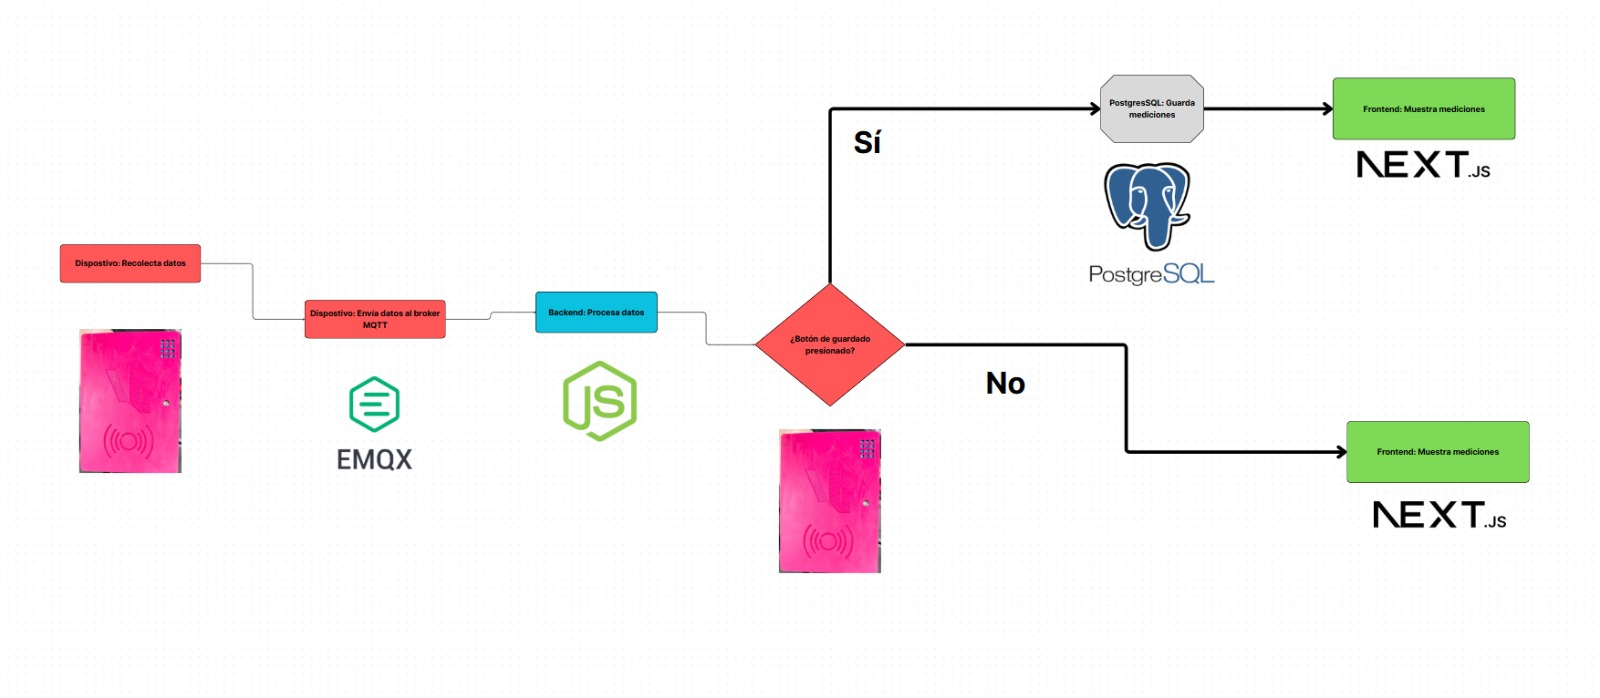
\includegraphics[width=0.95\textwidth]{../tesis/00Figuras/esquema.jpeg}
    \vspace{0.2cm}

    \footnotesize \textit{Flujo de datos: dispositivo ESP32 $\rightarrow$ broker MQTT $\rightarrow$ backend Node.js $\rightarrow$ PostgreSQL $\rightarrow$ frontend Next.js.}
\end{frame}

% =============================================================================
% SECCIÓN 4: METODOLOGÍA
% =============================================================================
\section{Metodología y Validación}

\begin{frame}{Enfoque de Investigación}
    Estudio aplicado, experimental, tecnociéntico e interdisciplinario.
    \vspace{0.3cm}
    \begin{itemize}
        \item \textbf{Enfoque:} Cuantitativo
        \item \textbf{Datos:} Series temporales IoT + modelado determinista + análisis predictivo
        \item \textbf{Horizonte:} Ciclos experimentales de 15 días en mesocosmos controlados
    \end{itemize}
\end{frame}

\begin{frame}{Fase I: Instrumentación IoT}
    Configuración y calibración del módulo de sensores:
    \vspace{0.3cm}
    \begin{itemize}
        \item Microcontroladores ESP32 con sensores NDIR para CO$_2$ y CH$_4$
        \item Curvas de calibración frente a concentraciones patrón
        \item Algoritmos de compensación cruzada por temperatura y humedad
        \item Buffer local (SD/Flash) + telemetría asincrónica MQTT
    \end{itemize}
\end{frame}

\begin{frame}{Fase II: Modelo Mecanicista}
    Formulación y parametrización del modelo EDO/DEB:
    \vspace{0.3cm}
    \begin{itemize}
        \item Adaptación del marco bioenergético de Eriksen (2022) para BSF
        \item Curva teórica de respiración como línea base de eficiencia máxima
        \item Supuesto de aerobiosis estricta
    \end{itemize}
\end{frame}

\begin{frame}{Fase III: Integración Híbrida}
    Desarrollo del algoritmo de estimación de estados:
    \vspace{0.3cm}
    \begin{itemize}
        \item RNA infiere biomasa larval a partir de variables operativas
        \item Integración dinámica como entrada al modelo mecanicista
        \item Corrección del error residual entre modelo y sensor
    \end{itemize}
\end{frame}

\begin{frame}{Fase IV: Métricas Ambientales}
    Validación de la utilidad para gestión ambiental:
    \vspace{0.3cm}
    \begin{itemize}
        \item Detección de eventos de anaerobiosis mediante CH$_4$
        \item Cuantificación del carbono emitido vs. estimado teóricamente
        \item Contraste de indicadores dinámicos frente a estimaciones estáticas tradicionales
    \end{itemize}
\end{frame}

\begin{frame}{Las Cuatro Fases (Diagrama)}
    \centering
    \begin{tikzpicture}[scale=0.8, transform shape,
        fase/.style={rectangle, rounded corners, draw, minimum width=2.4cm, minimum height=1.8cm, align=center, font=\small},
        flecha/.style={->, thick, >=stealth}]
        \node[fase, fill=green!10] (f1) at (0,0) {\textbf{I}\\Instrumentación\\IoT};
        \node[fase, fill=blue!10] (f2) at (3.2,0) {\textbf{II}\\Modelo\\DEB};
        \node[fase, fill=orange!10] (f3) at (6.4,0) {\textbf{III}\\Integración\\Híbrida};
        \node[fase, fill=red!10] (f4) at (9.6,0) {\textbf{IV}\\Métricas\\Ambientales};
        \draw[flecha] (f1) -- (f2);
        \draw[flecha] (f2) -- (f3);
        \draw[flecha] (f3) -- (f4);
        \draw[flecha, dashed, bend left=30] (f4.north) to node[above, font=\tiny] {Re-entrenamiento} (f3.north);
    \end{tikzpicture}
\end{frame}

\begin{frame}{Hipótesis y Criterios de Éxito}
    \centering
    \footnotesize
    \begin{tabular}{@{}llc@{}}
        \toprule
        \textbf{Hipótesis} & \textbf{Descripción} & \textbf{Criterio} \\
        \midrule
        H1 & Precisión sensores NDIR & MAPE $\leq$ 15\%, $R > 0.85$ \\
        H2 & Capacidad predictiva DEB & Tendencia base $R^2 > 0.70$ \\
        H3 & Refinamiento ML & Reducción $\geq$ 30\% error residual \\
        H4 & Detección anaerobiosis & Recall $>$ 80\% \\
        \bottomrule
    \end{tabular}
    \vspace{0.3cm}
    \normalsize
    H1--H3: condiciones de laboratorio (30$\pm$2°C, HR 60--70\%). H4: análisis de escenarios operativos.
\end{frame}

\begin{frame}{Contexto Experimental: Sede Palmira}
    \begin{itemize}
        \item \textbf{Ubicación:} Universidad Nacional de Colombia, Sede Palmira
        \item \textbf{Ecosistema:} Bosque tropical seco
        \item \textbf{Temperatura media anual:} 24°C
        \item \textbf{Condiciones de laboratorio:} Mesocosmos controlados
        \item \textbf{Variables controladas:} 30°C $\pm$2°C, HR 60--70\%
        \item \textbf{Ventana experimental:} Ciclos de 15 días
        \item \textbf{Frecuencia de muestreo:} Cada 30 min (sensores), biomasa cada 48h
    \end{itemize}
\end{frame}

\begin{frame}{Contexto Experimental (Mapa)}
    \centering
    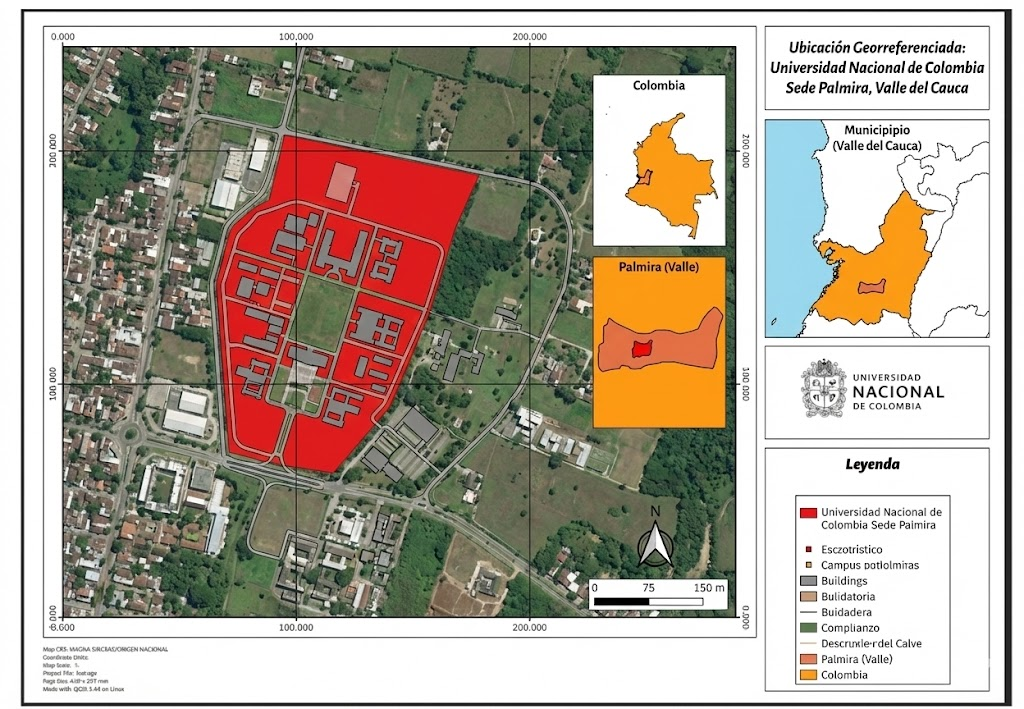
\includegraphics[width=0.65\textwidth]{../tesis/00Figuras/localizacion.jpg}
    \vspace{0.2cm}

    \footnotesize \textit{Ubicación georreferenciada del proyecto. Valle del Cauca, Colombia.}
\end{frame}

% =============================================================================
% SECCIÓN 5: APORTE Y ÉTICA
% =============================================================================
\section{Aporte y Responsabilidad}

\begin{frame}{Impacto 1: Factores de Emisión para IPCC}
    Generación de evidencia empírica para:
    \vspace{0.3cm}
    \begin{itemize}
        \item Establecer factores de emisión específicos para bioconversión con BSF
        \item Alinear la tecnología con marcos climáticos globales (IPCC Tier 3)
        \item Sustituir supuestos no verificados por datos medidos y modelados
    \end{itemize}
\end{frame}

\begin{frame}{Impacto 2: Optimización Operativa}
    La medición continua habilita la detección temprana de ineficiencias:
    \vspace{0.3cm}
    \begin{itemize}
        \item Sobrepoblación larval
        \item Exceso de humedad en el sustrato
        \item Deficiente aireación (formación de microambientes anaeróbicos)
    \end{itemize}
    \vspace{0.3cm}
    Cada condición subóptima reduce eficiencia de conversión y aumenta emisiones.
\end{frame}

\begin{frame}{Impacto 3: Trazabilidad MRV}
    Construcción de bases para certificación ambiental:
    \vspace{0.3cm}
    \begin{itemize}
        \item Metodologías de Medición, Reporte y Verificación (MRV)
        \item Alineación con estándares internacionales (Verra/VCS)
        \item Habilitación del acceso a mercados de carbono regulados
        \item Trazabilidad digital con sellado de tiempo (timestamping)
    \end{itemize}
\end{frame}

\begin{frame}{Protocolo de Respuesta Operativa}
    El sistema traduce predicciones en instrucciones concretas para el productor:
    \vspace{0.3cm}
    \begin{itemize}
        \item \textcolor{verdeOK}{\textbf{Verde (Normal):}} Emisiones dentro del rango aeróbico. Acumulación de créditos de carbono.
        \item \textcolor{naranjaAlerta}{\textbf{Ámbar (Preventivo):}} Tendencia al alza en la relación CO$_2$/O$_2$. Sugiere revisión de humedad.
        \item \textcolor{rojoAlerta}{\textbf{Rojo (Crítico):}} Detección de picos de CH$_4$. Intervención inmediata (volteo del sustrato).
    \end{itemize}
\end{frame}

\begin{frame}{Protocolo de Respuesta (Diagrama)}
    \centering
    \begin{tikzpicture}[scale=0.9, transform shape,
        estado/.style={rectangle, rounded corners, draw, minimum width=3.5cm, minimum height=1cm, align=center, font=\small\bfseries}]
        \node[estado, fill=verdeOK!20] (v) at (0,2) {VERDE\\Normal};
        \node[estado, fill=naranjaAlerta!20] (a) at (4.5,2) {ÁMBAR\\Preventivo};
        \node[estado, fill=rojoAlerta!20] (r) at (9,2) {ROJO\\Crítico};
        \node[below=0.3cm of v, font=\tiny, align=center] {Acumular\\créditos};
        \node[below=0.3cm of a, font=\tiny, align=center] {Revisar\\humedad};
        \node[below=0.3cm of r, font=\tiny, align=center] {Volteo\\inmediato};
        \draw[->, thick, >=stealth] (v) -- (a);
        \draw[->, thick, >=stealth] (a) -- (r);
    \end{tikzpicture}
    \vspace{0.3cm}

    \footnotesize \textit{La predicción como activador de control de procesos, no como dato pasivo.}
\end{frame}

\begin{frame}{Compromisos Ético-Epistemológicos}
    El sistema es una herramienta de soporte, no de sustitución del juicio técnico.
    \vspace{0.3cm}
    \begin{itemize}
        \item \textbf{Transparencia algorítmica (XAI):} Modelos mecanicistas integrados que permiten rastrear el ``porqué'' de cada predicción
        \item \textbf{Soberanía de datos:} Edge computing para que los datos sensibles permanezcan bajo control del productor
        \item \textbf{Compatibilidad con saberes:} La tecnología complementa el conocimiento empírico del manejo de residuos
    \end{itemize}
\end{frame}

% =============================================================================
% SECCIÓN 6: CIERRE
% =============================================================================
\section{Cierre}

\begin{frame}{Objetivo General}
    \centering
    \vspace{0.5cm}
    \Large
    ``Transformar la bioconversión de una caja negra biológica a un proceso \textbf{transparente}, tecnológicamente \textbf{viable} y verificable \textbf{climáticamente}.''
    \normalsize
    \vspace{0.5cm}
    \begin{itemize}
        \item Sistema híbrido a escala de laboratorio
        \item Métricas de desempeño ambiental aplicables a gestión de residuos
    \end{itemize}
\end{frame}

\begin{frame}{Cronograma y Presupuesto}
    \begin{itemize}
        \item \textbf{Horizonte temporal:} 42 meses (agosto 2023 -- enero 2027)
        \item \textbf{Presupuesto estimado:} 267 millones de pesos colombianos (COP)
        \item \textbf{Modelo de financiamiento:} Mixto (aporte institucional UNAL + recursos propios)
        \item \textbf{Retorno de inversión:} Sistema MRV validado habilita acceso a mercados de carbono
    \end{itemize}
\end{frame}

\begin{frame}{Cronograma (Diagrama)}
    \centering
    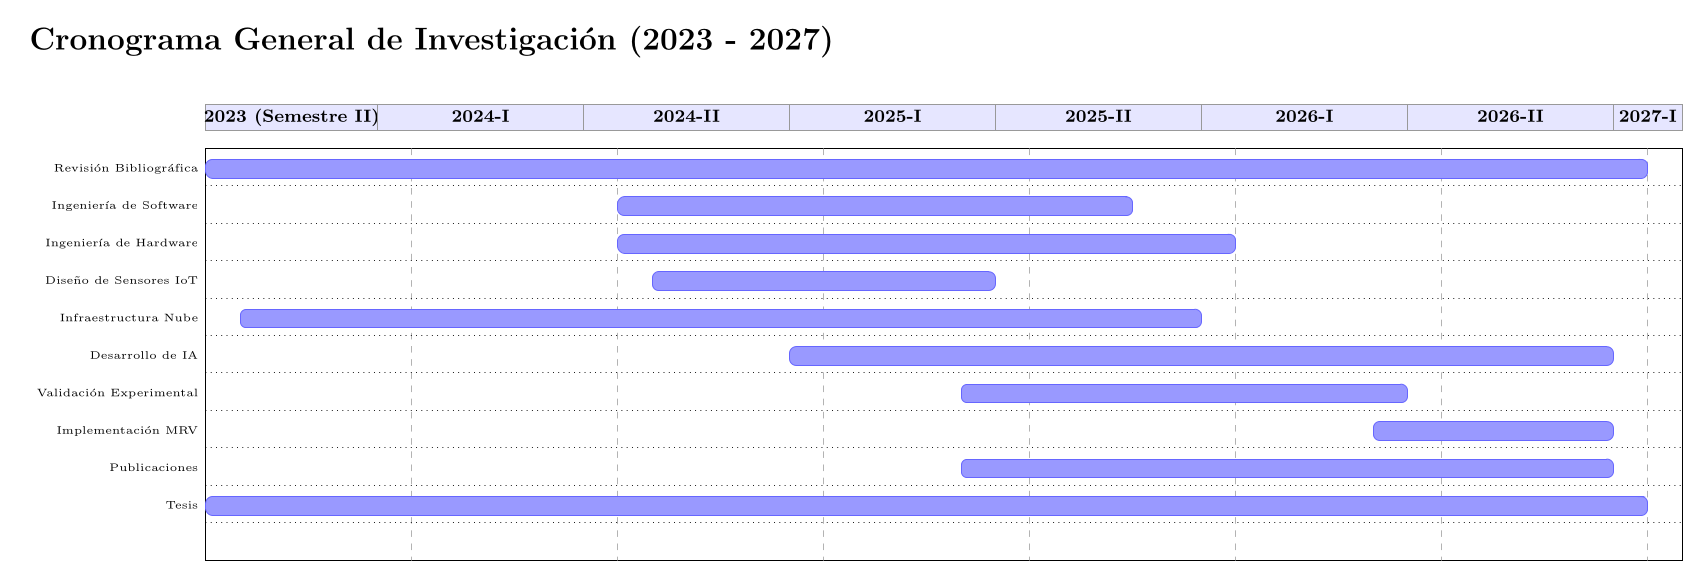
\includegraphics[width=0.85\textwidth]{../tesis/00Figuras/gant.png}
    \vspace{0.2cm}

    \footnotesize \textit{Cronograma de ejecución del proyecto doctoral.}
\end{frame}

\begin{frame}{}
    \centering
    \vspace{2cm}
    {\Huge \textbf{Gracias}}
    \vspace{1cm}

    {\large John Jairo Leal Gómez}
    \vspace{0.3cm}

    \texttt{jjlealg@unal.edu.co}
    \vspace{0.2cm}

    \footnotesize Doctorado en Estudios Ambientales\\
    Universidad Nacional de Colombia -- Sede Palmira
    \vspace{0.5cm}

    
\includegraphics[width=1.8cm]{../tesis/00Figuras/00f00EscudoUN2016.jpg}
\end{frame}

\end{document}
